Clase: 11/10/2022


\begin{teorema}[Taylor]
    Si $f(z)$ es analítica en el interior de un círculo $C$ con centro en $z=a$, $\forall z$ en el interior de $C$, se tiene que: 
    $$f(z)= \sum_{n=0}^\infty \underbrace{\frac{f^{(n)}(a)}{n!}}_{a_n}(z-a)$$
    \begin{dem}
        Sea 
        \begin{figure}[H]
           \centering
           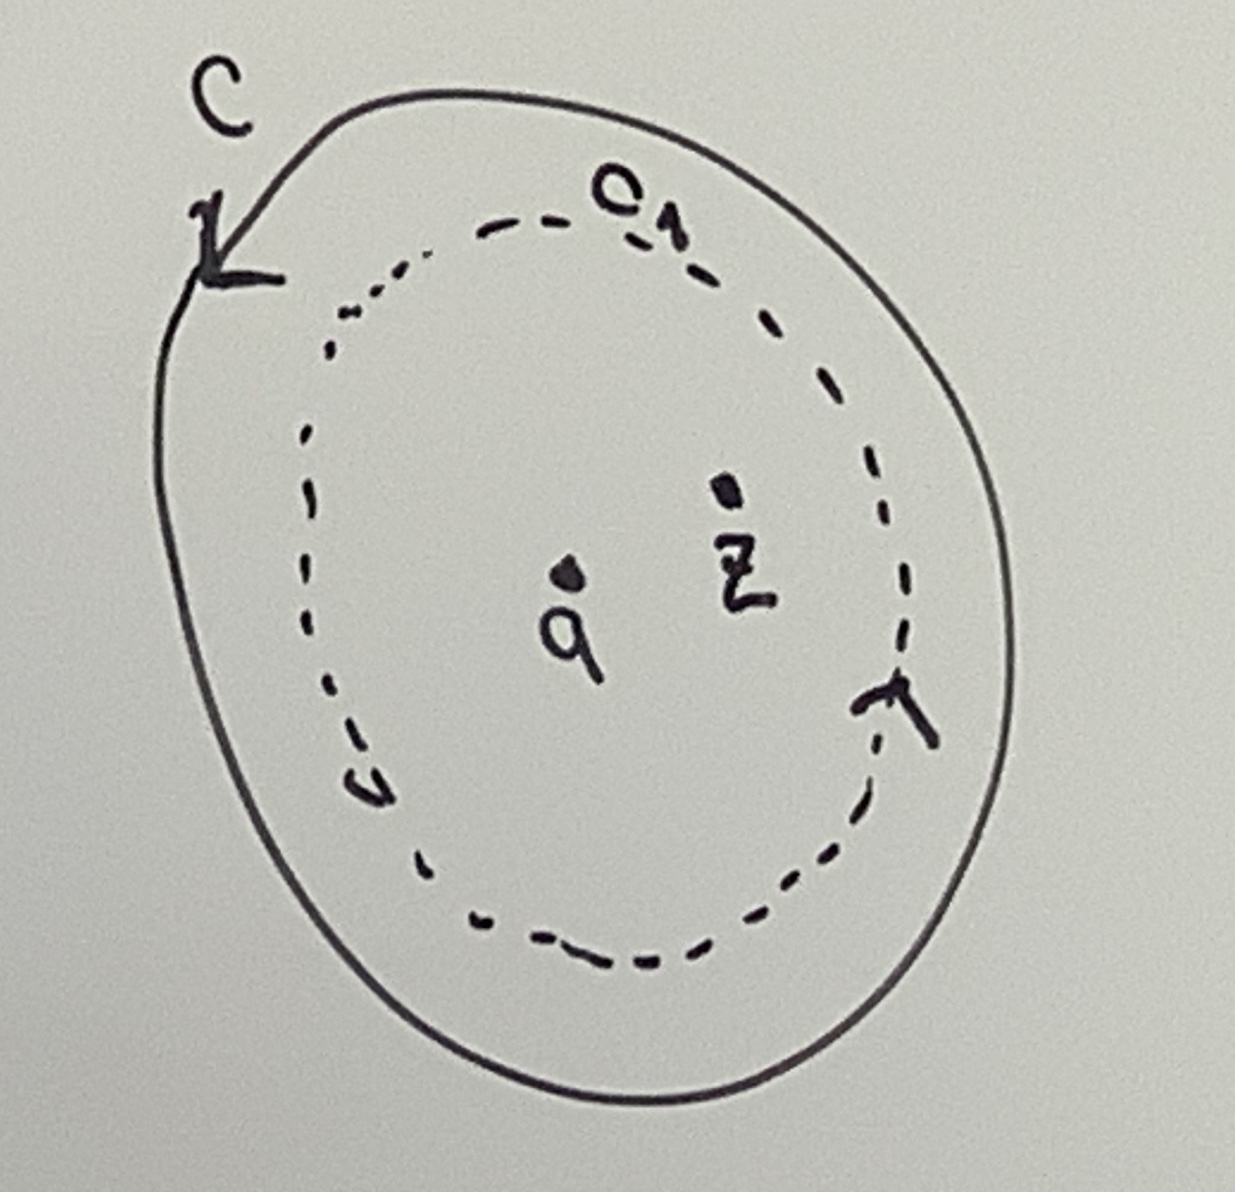
\includegraphics[scale=0.1]{imagenes/21.1.jpeg} 
        \end{figure}
        Sea $z$ un punto interior del círculo $c_1$ centrado en $a$ y contenido en el interior de $C$. 
        \begin{align*}
            f(z)&=\frac{1}{2\pi i}\int_{c_1}\frac{f(w)}{w-z}dz
        \end{align*}
        Sea 
        \begin{align*}
            \frac{1}{w-z}&=\frac{1}{(w-a)-(z-a)}\\
            &=\frac{1}{w-a}\left[\frac{1}{1-\left(\frac{z-a}{w-a}\right)}\right]\\
            &= \left|\frac{z-a}{w-a} \right|\\
            &= \frac{|z-a|}{|w-a|}<1
        \end{align*}
        Sea ahora
        \begin{align*}
            \frac{1-\left(\frac{z-a}{w-a}\right)^n}{1-\frac{(z-a)}{w-a}} &= 1+\left(\frac{z-a}{w-a}\right)
            +\cdots + \left(\frac{z-a}{w-a}\right)^{n-1}\\
            \frac{1}{1-\left(\frac{z-a}{w-a}\right)} &= 1+\left(\frac{z-a}{w-a}\right)+\left(\frac{z-a}{w-a}\right)^2 +\cdots \left(\frac{z-a}{w-a}\right)^{n-1}+\left(\frac{z-a}{w-a}\right)^n\cdot \frac{1}{1-\frac{z-a}{w-a}}\\
            \begin{split}
                \frac{1}{w-z}&=\frac{1}{w-a}\left[1+\left(\frac{z-a}{w-a}\right)+\left(\frac{z-a}{w-a}\right)^2 +\cdots + +\left(\frac{z-a}{w-a}\right)^{n-1}\right]+\\
                &+\left(\frac{z-a}{w-a}\right)^n\cdot\left(\frac{1}{w-z}\right)
            \end{split}\\
            &= \frac{1}{w-a}+\frac{(z-a)}{(w-a)^2}+\cdots + \frac{(z-a)^{n-1}}{(w-a)^n}+\left(\frac{z-a}{w-a}\right)^n\cdot \frac{1}{w-z}\\
            \begin{split}
            \frac{1}{2\pi i}\int_{c_1}\frac{f(w)}{w-z}dw&= \frac{1}{2\pi i}\int_{c_1}\frac{1}{w-a}dw+\frac{1}{2\pi i}\int_{c_1}\frac{(z-a)}{(w-a)^2}dw+\cdots +\\
            &+ \frac{1}{2\pi i}\int_{c_1}\frac{f(w)(z-a)^{n-1}}{(w-a)^n}dw+\frac{1}{2\pi i}\int_{c_1}\frac{\left(f(w)\frac{z-a}{w-a}\right)^n}{w-z}dw
            \end{split}\\
            f(z)&=f(a)+f'(a)(z-a)+\cdots + \frac{f^{(n-1)(a)}}{(n-1)!}(z-a)^{n-1}+R_n
        \end{align*}
        donde $$R_n=\frac{1}{2\pi i}\int_{c_1}\frac{f(w)(z-a)^n}{(w-z)(w-a)^n}dw$$
        A probar: si $n\to\infty\implies R_n\to 0$. Nótese que 
        \begin{align*}
            \left|\frac{z-a}{w-a}\right|^n =\mu^n <1
        \end{align*}
        Además, $|w-z|=|(w-a)-(z-a)|\geq |(w-a)|-|(z-a)|=r_1-|z_1-a|$
        Entonces, 
        $$\frac{1}{w-z}\leq \frac{1}{r_1-|z-a|}$$
        Como $f$ es continua sobre $c_1$, entonces $\exists M\geq 0\ni |f(w)|\leq M,\forall w\in c_1$.
        Entonces 
        \begin{align*}
            \left|r_n\right| &=\frac{1}{2\pi i}\left|\frac{f(w)}{w-z}\left(\frac{z-a}{w-a}\right)^ndw\right|\\
            &\leq \frac{1}{2\pi}\frac{M}{[r_1-(z-a)]}\cdot \mu^n(2\pi r_1)
        \end{align*}
        Cuando $n\to\infty 0$
    \end{dem}
\end{teorema}